\chapter{Súčasný stav problematiky}
\label{kap:stav}

Pri spracovaní informácie pomocou informačných a komunikačných technológií je potrebné, zabezpečiť prenos rôznych údajov medzi jednotlivými komponentami systému. Pri návrhu riešenia pre takúto komunikáciu je však potrebné, vzhľadom na konkrétne použitie, dbať aj na bezpečnosť údajov ako aj samotnej komunikácie. V dnešnej dobe sa často vyskytujú aj komerčne vyvinuté systémy, pri ktorých návrhu sa (často z dôvodu nedostatku financií alebo časového stresu) kladie malý, niekedy až žiadny dôraz na bezpečnosť riešenia, čo má za následok rôzne druhy zraniteľností vo výsledných, častokrát aj v certifikovaných, produktoch.

Takúto zraniteľnosť možno potom zneužiť a realizovať tak úspešný útok na daný systém. My sa v práci budeme venovať konkrétnym druhom útokov, ktorých cieľom je narušiť prebiehajúcu komunikáciu medzi dvomi časťami systému a tým dosiahnuť zmenu správania systému, ktorá v konečnom dôsledku umožní útočníkovi napríklad obísť bezpečnostný mechanizmus.

\section{Prehľad útokov na zariadenia} \label{kap1:sek:utoky}
Väčšinu útokov na zariadenia možno rozdeliť do troch kategórií \cite{mitmPCIe}.

\textbf{Útoky na softvérovej úrovni}, tiež SLA (Software Level Attacks), zneužívajú zraniteľnosti na úrovni operačného systému alebo aplikácie za účelom eskalácie privilégií. Hlavná výhoda týchto útokov je neobmedzená vzdialenosť útočníka a cieľového zariadenia \cite{mitmPCIe}. Nevýhodou pre útočníka je jednoduché nasadenie protiopatrení, ktoré možno vykonať aktualizáciou príslušného softvéru, ktorá zneužiteľnú zraniteľnosť opraví.

\textbf{Útoky na hardvérovej úrovni}, alebo HLA (Hardware Level Attacks), vytvárajú zraniteľnosti na zariadeniach, buď modifikáciou hardvéru, alebo iných faktorov, ktoré ovplyvňujú jeho správanie (napätie, elektromagnetické rušenie a pod.) \cite{mitmPCIe}. Výhodou takéhoto útoku sú takmer neobmedzené možnosti ako ovplyvniť správanie hardvéru, čo poskytuje veľkú flexibilitu. Takýto útok však vyžaduje fyzický prístup útočníka k zariadeniu. Navyše moderný hardvér disponuje fyzickými protiopatreniami, ktoré komplikujú, niekedy až úplne znemožňujú jeho ovplyvňovanie. Zraniteľnosti, ktoré umožňujú realizovať hardvérový útok je však náročné opraviť, nakoľko si vyžadujú výmenu hardvéru, ktorá vyžaduje často netriviálne náklady.

\textbf{Útoky na protokolovej úrovni}, PLA (Protocol Level Attacks), cielia na komunikáciou medzi entitami v systéme \cite{mitmPCIe}. Takéto útoky sa zameriavajú najmä na komunikáciu po sieti, často bezdrôtovej. Útoky tohto typu môžu byť vo všeobecnosti rôzne a náročnosť samotného útoku ako aj implementácia protiopatrenia závisí od zneužitej zraniteľnosti \cite{mitmPCIe}. V práci sa zameriame na konkrétny prípad hybridného útoku na protokolovej úrovni v kombinácií s útokom na hardvér a preskúmame možnosti jeho využitia.

\section{Man-in-the-middle útoky} \label{kap1:sek:mitm}
Man-in-the-middle (MITM) je spôsob útoku na komunikáciu prebiehajúcu po kanáli medzi dvoma entitami, pri ktorom útočník presmeruje komunikáciu z pôvodného kanálu na druhý kanál, ktorý je pod kontrolou útočníka. Takýto útok je často realizovaný transparentne z pohľadu účastníkov komunikácie  a vytvára tým zdanie, že účastníci sú spojený priamo. V skutočnosti však komunikácia prechádza cez tretiu entitu, ktorú má útočník pod kontrolou (napr. zariadenie, proces, systém). Tá je následne schopná, komunikáciu či už pasívne odpočúvať, alebo dokonca aktívne do komunikácie zasahovať. Schéma MITM útoku je znázornená na obrázku \ref{obr:mitm}.

\begin{figure}
    \centerline{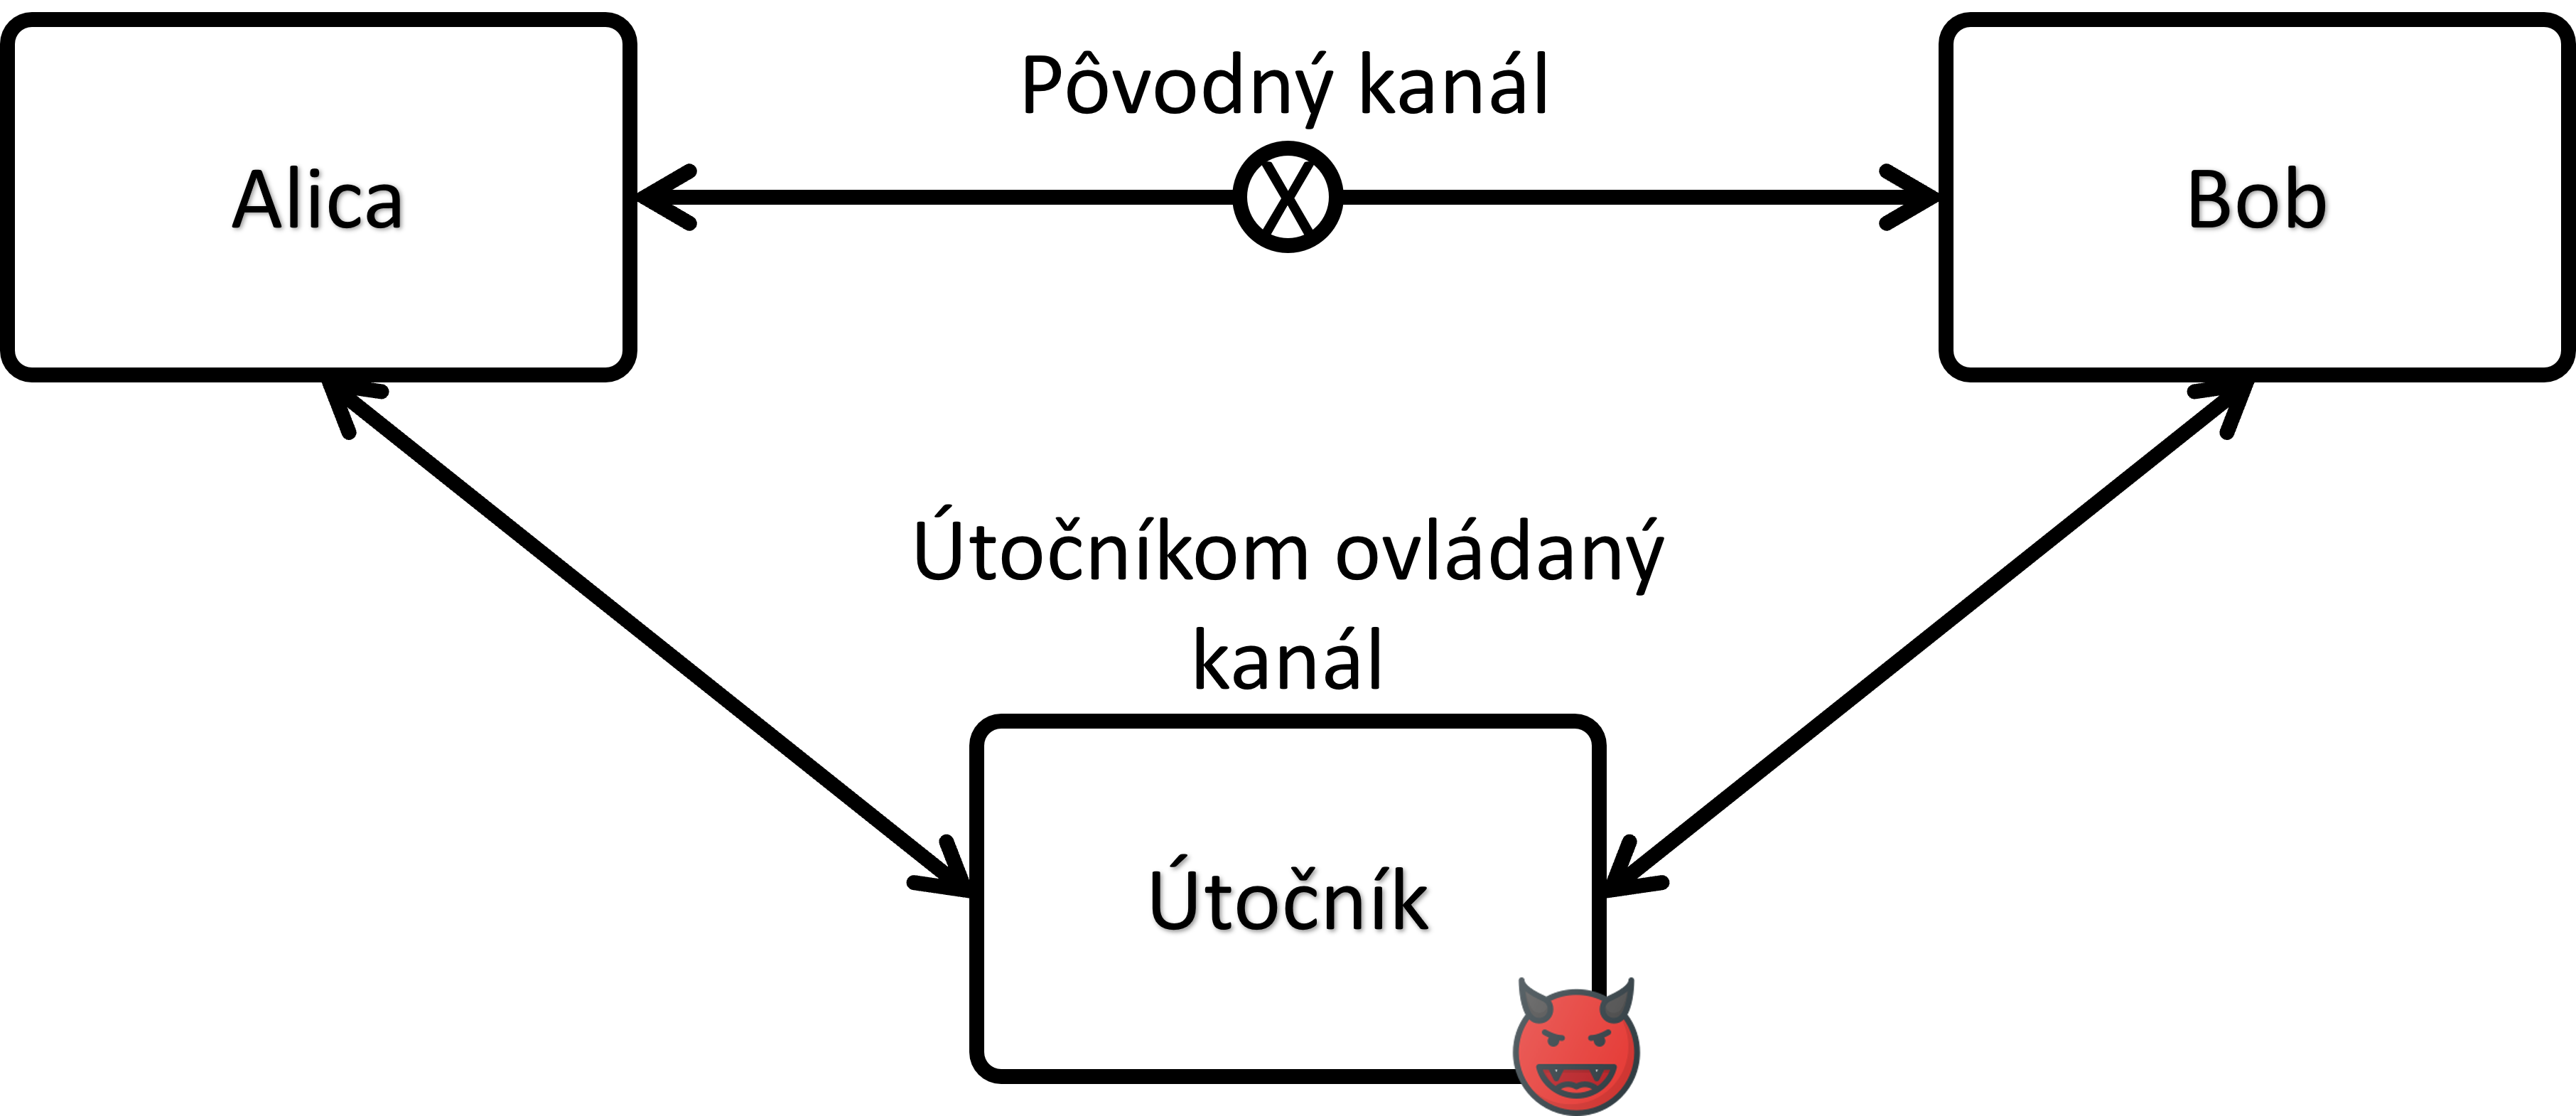
\includegraphics[width=0.75\textwidth]{images/mitm.png}}
    \caption[Schéma MITM útoku]{Schéma MITM útoku.}
    \label{obr:mitm}
\end{figure}

Bezpečnostných opatrení, ktoré znemožňujú týmto spôsobom útočiť na komunikáciu je viacero, ich princíp sa však opiera o tri základné požiadavky informačnej bezpečnosti. Zabezpečujú dôvernosť prenášanej informácie pre znemožnenie pasívneho odpočúvania, integritu a autenticitu za účelom znemožnenia aktívneho zasahovania do komunikácie, prípadne aj detekciu pokusu o MITM útok \cite{mitmTheory}. My sa v práci nebudeme venovať všeobecným MITM, ale budeme sa sústrediť na konkrétnejší scenár MITM útoku a možnosti jeho realizácie.

\subsection{Hardvérové Man-in-the-middle útoky}
MITM útoky sú často uvažované v prostredí sieťovej komunikácie, kde má útočník prístup k niektorému zo zariadení podieľajúcich sa na prenose informácie po sieti, napr. smerovač (angl. router) \cite{mitmTheory}. MITM útok je však oveľa všeobecnejší a jeho techniku možno aplikovať prakticky v akomkoľvek scenári, kde prebieha komunikácia medzi dvoma entitami. Pomerne novou a nie veľmi preskúmanou myšlienkou, ktorá využíva útok typu MITM je útok na komunikáciu prebiehajúcu po zbernici medzi jednotlivými hardvérovými komponentami, napríklad ovplyvnenie komunikácie medzi CPU a pamäťou. Dôležitý predpoklad je prístup ku kanálu (alebo aspoň jeho časti), po ktorom prebieha komunikácia, teda v tomto prípade fyzický prístup ku zbernici.

Tento predpoklad je v poslednej dobe stále častejšie naplnený. Situácia, kedy má útočník fyzický prístup k zariadeniu je najčastejšie pri využití vnorených (angl. embedded) zariadení. Tie sa dnes čoraz častejšie využívajú na obsluhu rôznych systémov ako napríklad bezpečnostné kamery, inteligentné zámky, čipové karty a pod. Takýto typ MITM útoku sa v literatúre zvykne označovať ako hardvérový MITM útok.

\section{Známe príklady útokov} \label{kap1:sek:priklady}
Hardvérový MITM útok je pomerne nový koncept, ktorý sa dostal do pozornosti v~posledných rokoch, existuje už však viacero prác, ktoré sa takýmito útokmi zaoberali \cite{mitmPCIe, mitmTouch, mitmCAN, mitmI2C, mitmSPI}.

\subsection{Útok na odomknutie smarfónu}
Jednou z prvých prác, ktorá demonštrovala úspešný hardvérový MITM útok bol útok, ktorý umožnil obísť obmedzený počet pokusov na odomknutie
smartfónu \cite{mitmPCIe}. Následne bolo možné vykonať útok hrubou silou -- úplným preberaním z množiny slov  pevnej dĺžky nad desiatkovými číslicami.

Princíp útoku spočíval v ovplyvnení komunikácie medzi CPU a externou energeticky nezávislou (angl. non-volatile) pamäťou, ktorá obsahovala údaje o zostávajúcom počte pokusov. Komunikácia medzi CPU a pamäťou bola síce šifrovaná, ale útok zneužíval fakt, že posielané správy neboli označené jedinečným identifikátorom, napríklad časovou pečiatkou. To umožnilo vykonať útok opakovaním správy s informáciou o zostávajúcom počte pokusov, ktorá prichádzala z pamäte do CPU.

Útok bolo potom možné implementovať nasledovne: Útočník pripojil tretie zariadenie (realizované pomocou FPGA) na zbernicu medzi CPU a pamäťou. Toto zariadenie bolo schopné transparentne preposielať prebiehajúcu komunikáciu a súčasne analyzovať preposielané rámce. Štatistickou analýzou bolo možné po niekoľkých pokusoch identifikovať dvojicu správ (požiadavka -- odpoveď), ktorej súčasťou bola odpoveď prichádzajúca z pamäte obsahujúca zostávajúci počet pokusov. Túto správu zariadenie následne uložilo do lokálnej pamäte a na nasledujúcu požiadavku od CPU odpovedalo rovnakou správou, miesto toho, aby komunikáciu preposlalo skutočnej pamäti. Výsledkom bolo, že zostávajúci počet pokusov sa nedekrementoval a CPU umožnilo opäť zadať heslo.

\subsection{Útok výmenou dotykovej obrazovky}
Veľká časť smartfónov, tabletov, notebookov, či iných zariadení považuje hardvérové komponenty inštalované pri výrobe automatiky za dôveryhodné \cite{mitmTouch}. Takýto bezpečnostný prístup sa na prvý pohľad môže zdať zmysluplný, faktom však je, že aj fyzicky interné zariadenia v rámci systému môžu byť niekedy pod kontrolou útočníka. Zaujímavý útok, ktorý zneužil tento fakt, bol opäť útok na smartfón, ktorý tentokrát výmenou dotykovej obrazovky za obrazovku úmyselne pripravenú útočníkom, umožnil vykonávať útočníkom kontrolované operácie nad príkazmi zadávanými používateľom do obrazovky.

Náhradná obrazovka bola následne schopná pasívne odpočúvať vstup od používateľa, vykonávať operácie v mene používateľa a dokonca zneužitím ďalších zraniteľností prítomných v jadre operačného systému získať administrátorské práva a tým aj úplnú kontrolu nad zariadením \cite{mitmTouch}. Autori zároveň poukazujú na realistický scenár tohto útoku, odvolávajúc sa na častú výmenu poškodených obrazoviek službami poskytovanými od neautorizovaných servisov. Tie sú často preferovanou voľbou zákazníkov s dôvodu nižších nákladov na opravu.

\subsection{Útoky na CAN zbernicu}
V dnešnej dobe je väčšina komponentov automobilov riadená mikrokontrolérmi alebo inými riadiacimi jednotkami. Pre zabezpečenie komunikácie medzi týmito jednotkami sa v automobiloch zvyčajne využíva tzv. CAN (Controller Area Network) zbernica. Pri vývoji CAN zbernice bolo hlavnou požiadavkou spoľahlivosť a zabezpečenie fyzickej bezpečnosti počas prevádzky vozidla. Moderné vozidlá však majú dnes množstvo rozhraní, prostredníctvom ktorých sú prepojené s okolitým svetom, čo môže umožniť prístup útočníkovi k vnútornej sieti prepájajúce riadiace jednotky vozidla (zvyčajne realizovanej CAN zbernicou) \cite{mitmCAN}.
Tejto problematike sa preto venovala práca, ktorej výsledkom bolo vyvinutie univerzálneho zariadenia, ktoré je možné použiť na implementáciu hardvérového MITM útoku na CAN zbernicu \cite{mitmCAN}. Toto zariadenie je možné naprogramovať, aby nad prebiehajúcou komunikáciou realizovalo rôzne operácie (napr. opakovanie správy, blokovanie komunikácie, cielená modifikácia správy a pod.).

\subsection{Ďalšie útoky}
Existuje aj niekoľko ďalších prác venujúcich sa hardvérovým MITM útokom \cite{mitmI2C, mitmSPI}. Tie sú najmä pasívneho charakteru (napr. odpočúvanie komunikácie). Všetky tieto útoky, rovnako ako predošle spomenuté, zneužívajú fakt, že pri návrhu komunikácie medzi hardvérovými komponentami sa často očakáva dôveryhodné prostredie (zbernica), v ktorom komunikácia prebieha. Práce poukazujú aj na to, že v poslednej dobe je tento predpoklad čoraz zriedkavejšie pravdivý.

\section{Niektoré známe protiopatrenia} \label{kap1:sek:protiopatrenia}
Pri klasickom MITM scenári po sieti spočívajú protiopatrenia v zabezpečení integrity a autentickosti prebiehajúcej komunikácie prostredníctvom kryptografie, napr. použitím TLS protokolu \cite{mitmTheory}. V hardvérovom scenári je však takýto druh protiopatrení problém, z dôvodu obmedzenej výpočtovej kapacity. Štandardy pre prenos dát po zberniciach špecifikujú pomerne veľké rýchlosti prenosu, rádovo od Mb/s až po stovky Gb/s \cite{i2cBus, mitmPCIe}. To znamená, že navrhnuté protiopatrenie musí umožniť dostatočne rýchle spracovanie správy, ktoré bude v súlade so štandardom. Niekedy to môže znamenať potrebu spracovať správu rádovo za niekoľko mikrosekúnd \cite{mitmPCIe}.

Existujúce protiopatrenia voči hardvérovým MITM útokom sa preto väčšinou zameriavajú na aktívnu detekciu takéhoto útoku, ktorú možno vykonávať súčasne s prebiehajúcou komunikáciou. Pre vykonanie samotného MITM útoku na zbernici je tiež potrebné vykonať určité operácie, ktoré môžu spôsobiť odchýlku v prenosovej rýchlosti. Túto odchýlku je možné po niekoľkých meraniach detegovať a následne vyhlásiť chybu v komunikácií.

\section{Motivácia a ciele práce}
Vo všetkých spomenutých prácach autori poukazujú na náročnosť implementácie hardvérového MITM útoku z dôvodu obmedzenej výpočtovej kapacity \cite{mitmPCIe, mitmCAN, mitmTouch}. Podobne ako pri implementácií spomenutých protiopatrení, aj útočník nemôže vykonávať zložitejšie výpočty, ktoré by príliš spomalili komunikáciu. Pri väčšine implementácií je síce možné mierne prekročiť limity pre danú zbernicu dané štandardom, pokiaľ je však komunikácia spomalená príliš, jednotlivé zariadenia môžu vyhlásiť chybu v komunikácií, čo by útok znemožnilo.

Preto je hlavným cieľom práce preskúmať možnosti implementácie hardvérového MITM útoku na komunikačné zbernice. Najzaujímavejším aspektom je práve overenie ako výpočtovo zložité zásahy do komunikácie bude možné realizovať v reálnom čase. Spomínané útoky využívali na implementáciu útočiaceho zariadenia tzv. programovateľné hradlové pole, ďalej len FPGA (Field-Programmable Gate Array).

FPGA je integrovaný logický obvod, ktorý možno nakonfigurovať, aby sa správal ako konkrétny logický obvod realizovaný priamo hardvérom. Výhoda tohto prístupu oproti programu interpretovaného procesorom je práve rýchlosť, keďže FPGA neinterpretuje inštrukcie, ale realizuje operácie priamo nakonfigurovaným obvodom.

Očakávame preto, že implementácia MITM útoku pomocou FPGA nám umožní vykonávať rádovo zložitejšie operácie v porovnaní s klasickým prístupom. Ďalším zaujímavým cieľom je práve experimentálne porovnanie, ako veľmi nám použitie FPGA umožní zdvihnúť výpočtový výkon oproti prístupu s procesorom, respektíve, či je vôbec možné realizovať hardvérový MITM útok použitím programu interpretovaného, napr. mikrokontrolérom. Dôvodom pre voľbu tohto druhého prístupu môžu byť napríklad nižšie finančné náklady ako pri implementácií pomocou FPGA.

Ďalším cieľom práce je overenie možnosti protiopatrení na implementované útoky použitím vhodných kryptografických primitív. Neočakávame, že použitie výpočtovo zložitejších kryptografických schém, ako napríklad asymetrické šifrovanie, či digitálne podpisy bude možné pri dodržaní rýchlosti komunikácie definovanej štandardom zbernice. Niektoré výpočtovo ľahšie konštrukcie, napríklad použitie PUF (Physical Unclonable Function) na implementáciu Challange-Response protokolu, však môžu byť vhodným kandidátom na zabezpečenie komunikácie. Možnosti aplikácie takéhoto protiopatrenia je však potrebné overiť.

V práci sa zameriame na konkrétne zbernice (napr. I2C, SPI) a cieľom útoku bude komunikácia medzi rôznymi hardvérovými komponentami (napr. CPU -- EEPROM a pod.)